\section{CoReGraph}

\begin{figure}[t]
  \centering
  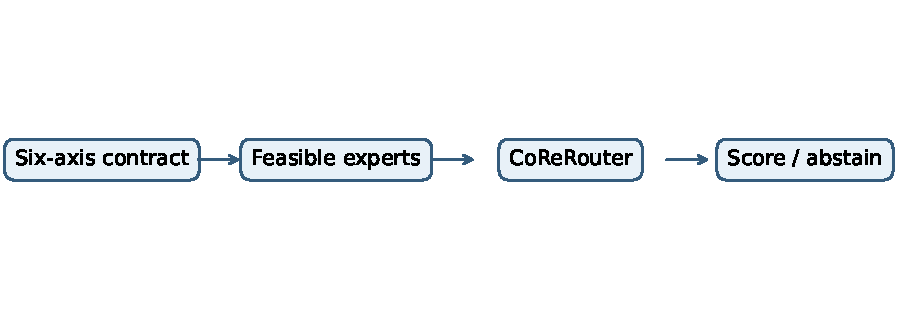
\includegraphics[width=\linewidth]{figures/figure_1_system_schematic.pdf}
  \caption{CoReGraph execution path. This is a system schematic, not an
  empirical result. Feasibility is imposed before routing, and no-feasible-
  expert cases abstain.}
  \label{fig:system}
\end{figure}

\paragraph{Factorised contract encoder.}
Each categorical coordinate has an embedding with an unknown token. Continuous
budget, memory, latency, and window values are concatenated after scaling.
Optional pairwise dot-product interactions capture low-order composition.
Axis dropout and bounded contract noise prevent brittle dependence on complete
metadata. An atomic contract-ID encoder and a no-contract encoder serve as
baselines; the atomic encoder maps held-out IDs to an unknown token.

\paragraph{Label-free diagnostics.}
The router can consume expert scores, confidence, entropy, score and rank
disagreement, visible degree and isolation, missingness, temporal instability,
graph density, unlabelled score drift, predicted prevalence, cost, and
availability. Every diagnostic declares its graph view, granularity, target
access, and label requirement. Label-dependent graph-harm diagnostics are
source-only and cannot enter target inference.

\paragraph{Masked routing and safe behaviour.}
CoReRouter scores expert tokens using a linear, MLP, or small attention router.
Unavailable experts receive negative-infinite routing logits and exactly zero
weight. If no expert is feasible, the system abstains. Otherwise it can fall
back to a feature-only expert, the fixed source-validation winner, a static
average, or a top-two mixture. Outputs include weights, selected expert,
abstention probability, entropy, expected compute, and an explanation record.

\paragraph{Objective.}
For source contract groups, the configurable loss is
\[
 \mathcal L =
 \lambda_{\mathrm{avg}}\mathcal L_{\mathrm{pred}}+
 \lambda_{\mathrm{reg}}\operatorname{CVaR}_\alpha(\mathrm{Reg}_c)+
 \lambda_{\mathrm{bud}}\mathcal L_{\mathrm{budget}}+
 \lambda_{\mathrm{stab}}\mathcal L_{\mathrm{stability}}+
 \lambda_{\mathrm{cost}}\mathcal L_{\mathrm{compute}}+
 \lambda_{\mathrm{cal}}\mathcal L_{\mathrm{calibration}}.
\]
The budget term is a smooth top-$K$ surrogate; we do not claim exact
optimisation of discontinuous Recall@$K$. Stability covers contract
perturbations, score noise, and availability masks.

\begin{figure}[t]
  \centering
  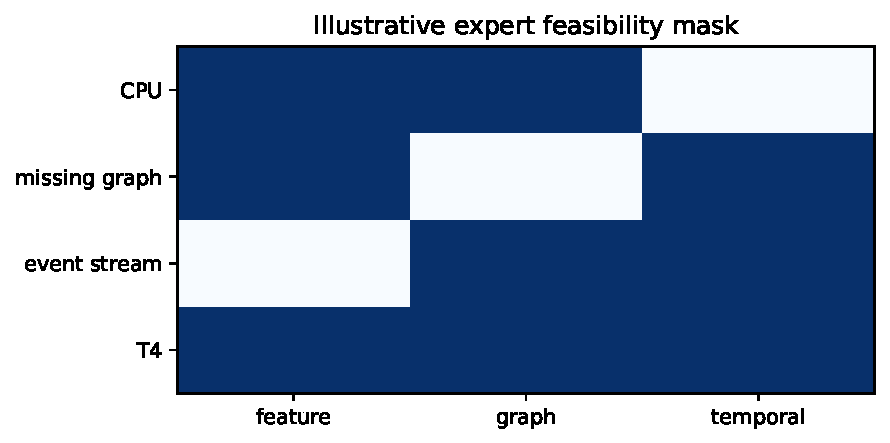
\includegraphics[width=.72\linewidth]{figures/figure_3_resource_mask.pdf}
  \caption{Illustrative feasibility masks under four resource/visibility
  settings. Shading is schematic and contains no measured availability.}
  \label{fig:resource-mask}
\end{figure}
